% // Esta apresentação -- desenvolvida por Sérgio Mendonça -- está licenciada
% // com uma Licença Creative Commons -- Atribuição (BY) -- Não Comercial (NC)
% // -- Compartilha Igual (SA) 4.0 Internacional. Baseado no trabalho
% // disponível em: https://github.com/sftom/templates/ufpe/presentation
% //
% // +---------------------------------------------------+
% // | Universidade Federal de Pernambuco                |
% // | Centro de Tecnologia e Geociencias                |
% // | Programa de Pos-Graduacao em Engenharia Eletrica  |
% // | Sergio Mendonca -- http://bcc.uag.ufrpe.br/~sftom |
% // +---------------------------------------------------+

\documentclass{beamer}
\definecolor{links}{HTML}{2A1B81}
\hypersetup{colorlinks,linkcolor=,urlcolor=links}
\usepackage[brazil]{babel}   
\usepackage[utf8]{inputenc} 
\usepackage{lmodern}

\title[Metodologia Científica]{Metodologia Científica - Getting Things Done}
\subtitle[GTD]{A arte de fazer acontecer}
%\author[sergio.mendonca.pro]{\url{http://sergio.mendonca.pro}}
\author[Sérgio Mendonça]{\href{http://bcc.uag.ufrpe.br/\~sftom}{Sérgio Francisco Tavares de Oliveira Mendonça}}
\institute[UFPE-PPGEE]{


\includegraphics[width=4em]{img/logo_ufpe.png}

\textbf{Universidade Federal de Pernambuco}\\Centro de Tecnologia e Geociências\\Programa de Pós-Graduação em Engenharia Elétrica\\\textbf{Metodologia Científica}\\Professora Fernanda Maria Ribeiro de Alencar\\ \url{http://bcc.uag.ufrpe.br/\~sftom}}
%\date{29 de setembro de 2014}

\usetheme{CambridgeUS}\usecolortheme{beaver}

\begin{document}

%\maketitle

%capa (slide de título)
\begin{frame}[plain]
    \titlepage
\end{frame}


\begin{frame}
\frametitle{Sumário}
\setcounter{tocdepth}{3}
\tableofcontents
\end{frame}
\pgfdeclareimage[height=1.2cm]{logo}{img/logo_ufpe-ctg}
\logo{\pgfuseimage{logo}}

\AtBeginSection[]{
\begin{frame}
\frametitle{Agenda}
\tableofcontents[currentsection]
\end{frame}
}


\section{A sua mente}

\begin{frame}[t]\frametitle{Produtividade vs. Tralha}
    
	Como podemos ser produtivos com tantas coisas para fazer?

\end{frame}

\begin{frame}[t]\frametitle{Dinâmico vs. Estático}
    \begin{itemize}
    	\item GTD
    		\begin{itemize}
    			\item \textbf{Estático}: Coletar e FAZER
    			\item \textbf{Dinâmico}: Decidir e Revisar
    		\end{itemize}
    	\item Scrum
    		\begin{itemize}
    			\item \textbf{Estático}: Planejamento e retrospectiva
    			\item \textbf{Dinâmico}: \textit{Sprint}
    		\end{itemize}
    	\item Pomodoro
    		\begin{itemize}
    			\item \textbf{Estático}: 25 minutos
    			\item \textbf{Dinâmico}: 5 minutos de intervalo
    		\end{itemize}
    \end{itemize}
\end{frame}

\begin{frame}[t]\frametitle{Elementos iniciais}
\begin{itemize}
	\item Elementos-chave:
	\begin{itemize}
		\item controle
		\item perspectiva
	\end{itemize}
	\item \textit{Loops} abertos e incompletos, geralmente, tomam a nossa atenção 
	\item Precisamos identificar as coisas que nos fazem ``tocar o sino''
\end{itemize}
\end{frame}

\begin{frame}[t]\frametitle{Gerenciando Compromissos}
\begin{itemize}
	\item Se está em sua mente, sua mente não está clara, livre!
	\item Qual é o compromisso e o que deve ser feito?
	\item Organize lembretes de seu plano de ação e livre o seu cérebro de se manter a par de tudo
\end{itemize}
\end{frame}

\section{Fluxo de Trabalho}

\begin{frame}[t]\frametitle{Fases do GTD}
    \begin{itemize}
    	\item Coletar
    	\item Processar
    	\item Organizar
    	\item Revisar
    	\item Fazer
    	%\begin{block}{\textit{Swarm Intelligence}}é utilizado para descrever qualquer tentativa de projetar algoritmos ou dispositivos distribuídos voltados à solução de problemas inspirados pelo comportamento de insetos sociais
    	%\end{block}

    \end{itemize}
\end{frame}

\begin{frame}[t]\frametitle{Coletar}
	\begin{itemize}
	 	\item Capturar tudo o que você precisa controlar ou lembrar ou agir no que Allen chama de balde ou caixa de entrada;
		\item Retirar tudo de sua cabeça e deixar em seu dispositivo de coleta, pronto para processamento;
		\item Todas as caixas de entrada devem ser processadas pelo menos uma vez por semana.
	 \end{itemize} 
\end{frame}

\begin{frame}[t]\frametitle{Processar}
    \begin{itemize}
    	\item Inicie de cima, do topo.
		\item Lide com um item de cada vez.
		\item Nunca devolva um item à caixa de entrada.
		\item Se um item requer uma ação.
		\begin{itemize}
			\item Faça (se durar menos de dois minutos).
			\item Delegue ou adie.
		\end{itemize}
		\item Se não
		\begin{itemize}
			\item Arquivo ou referência.
			\item Delete.
			\item Incube-o para uma possível ação posteriormente.
		\end{itemize}
    \end{itemize}
\end{frame}

\begin{frame}[t]\frametitle{GTD Workflow}
\begin{figure}[tb]
	\begin{center}
		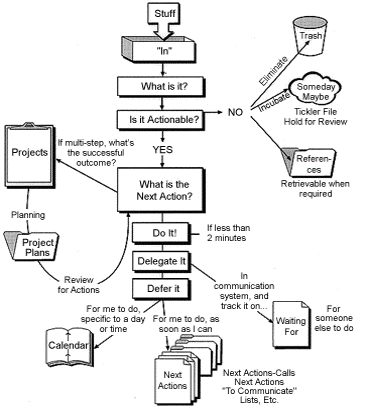
\includegraphics[width=0.45\linewidth]{img/workflow-gtd.png}
	\end{center}
	\caption{GTD Workflow}
	\label{fig:workflow-gtd}
\end{figure}
\end{frame}

\begin{frame}[t]\frametitle{Organizar}
	\begin{itemize}
		\item \textbf{Próximas ações} - Para cada item que exigir sua atenção, decida qual será a próxima ação que você pode tomar fisicamente nele
		\item \textbf{Projects} - Cada malha aberta que exige mais do que uma ação física para conseguir se tornar um \textbf{projeto}

		\item \textbf{Aguardando} - Quando você delegou uma ação para alguém ou esteja esperando por algum evento externo antes que você pode mover um projeto para a frente, \textbf{Someday/Maybe} - coisas que você quer fazer, em algum momento, mas não é certo agora
	\end{itemize}
\end{frame}

\begin{frame}[t]\frametitle{Revisar}
    \begin{itemize}
    	\item Reveja as suas listas de ações e lembretes diariamente

		\item Semanalmente, reveja todas as suas ações em circulação, projetos e itens à espera

		\item Crie um arquivo de referência rápida, a fim de ajudar a refrescar sua memória
    \end{itemize}
\end{frame}

\begin{frame}[t]\frametitle{Fazer}
	Critérios para Ações
    \begin{itemize}
    	\item Contexto
    	\item Tempo disponível
    	\item Energia
    	\item Prioridades
    \end{itemize}
\end{frame}

\begin{frame}[t]\frametitle{Perspectivas em 6 níveis}
\begin{enumerate}
	\item Ações atuais (correntes)
	\item Projetos atuais (correntes)
	\item Áreas de responsabilidades
	\item Metas anuais
	\item Visão em 5 anos
	\item Metas de vida
\end{enumerate}
\end{frame}

% \begin{frame}[t]\frametitle{Mente limpa como a água}
%     \begin{itemize}
% 		\item Para muitas pessoas que estão sobrecarregadas e estressadas ​​- este sistema é um avanço real
%     	\item As pessoas que tem muitas coisas em suas mentes, tenta se lembrar das coisas, muitas vezes tem dificuldade em pensar de forma criativa ou produtiva
%     	\item Quando as coisas estão fora de sua mente, é possível que você libere uma pessoa produtiva
%     	\item É provável que você vai dormir melhor e encontrar tempo para fazer coisas que você não poderia antes
%     \end{itemize}
% \end{frame}

\section{Ferramentas GTD} % (fold)
\label{sec:gtd_tools}

% section gtd_tools (end)
\begin{frame}[t]\frametitle{Mais ferramentas}
\begin{itemize}
	\item Tips and Tools from www.davidco.com
	\item Lifehacker.com
	\item Getting Things Done Outlook Add-In 
	\begin{itemize}
		\item http://gtdsupport.netcentrics.com
	\end{itemize}
	\item GTD for Lotus Notes
	\item GTD for Blackberry
	\begin{itemize}
		\item www.blackberryinsight.com
	\end{itemize}
\end{itemize}
\end{frame}

\section{Referências} % (fold)
\label{sec:references}

% section references (end)

\begin{frame}[t]\frametitle{GTD References \& Books}
    
\begin{figure}[tb]
	\begin{center}
		
\includegraphics[width=0.38\linewidth]{img/gtd-book.png}
	\end{center}
	\caption{Allen, David - Getting Things Done}
	\label{fig:figure1}
\end{figure}

\end{frame}

 \begin{frame}[c]\frametitle{Creative Commons Licence}
     \begin{figure}[ht]
          \centering
          \caption{\label{fig:by-nc-sa} Creative Commons Licence}
          
\includegraphics[width=0.3\textwidth]{./img/by-nc-sa.jpg}
      \end{figure} 
      Esta apresentação -- desenvolvida por Sérgio Mendonça -- está licenciada com uma Licença Creative Commons -- Atribuição (BY) -- Não Comercial (NC) -- Compartilha Igual (SA) 4.0 Internacional. Baseado no trabalho disponível em: \url{https://github.com/sftom/templates/ufpe/presentation}
 \end{frame}


\end{document}